\documentclass{article}
\usepackage[T1]{fontenc}
\usepackage{lmodern}
\usepackage{graphicx}
\usepackage{amsmath,amssymb}
\usepackage[a4paper,margin=2cm]{geometry}
\usepackage[absolute,overlay]{textpos}
\setlength{\TPHorizModule}{1mm}
\setlength{\TPVertModule}{1mm}
\usepackage[indonesian]{babel}
\usepackage{hyperref}
\setlength{\emergencystretch}{2em}
% unit: Halaman 6

\begin{document}

% === Halaman 6 (llm) ===

Pernah terima surel (\textit{e-mail}) dari orang tak dikenal dan mengandung \textit{file attachment} berupa gambar seperti di bawah ini?

\vspace{10mm}

\textbf{\color{red}HATI-HATI!!!!!!!!!!!}

% deskripsi: Screenshot contoh email phishing yang berisi lampiran gambar ucapan Tahun Baru 2016 dari 'Institute of Research Engineers and Doctors'.
% bbox normalisasi: [0.1780, 0.2760, 0.6540, 0.8730]
\begin{textblock*}{99.96mm}(37.38mm,81.97mm)
\noindent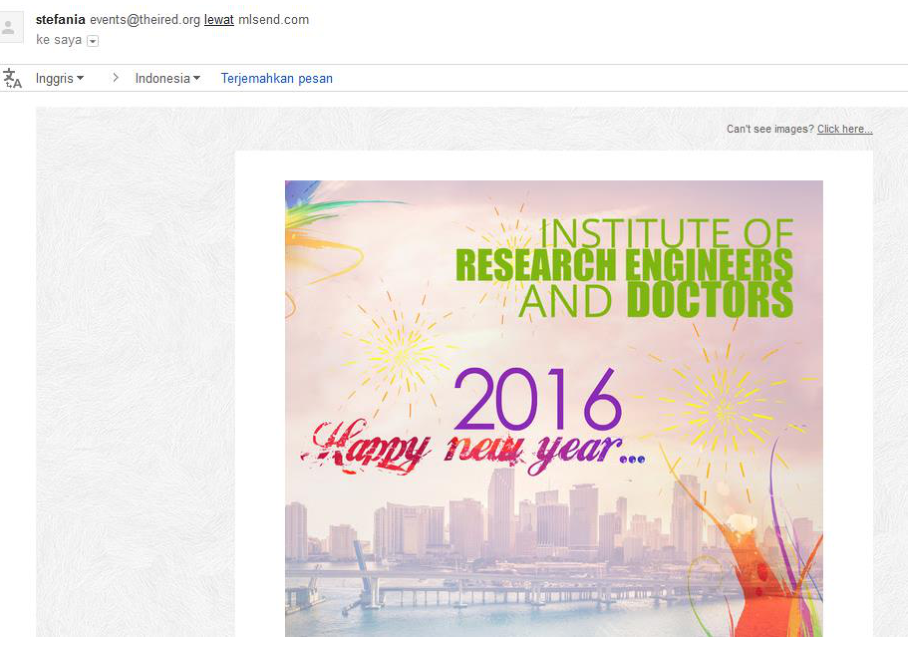
\includegraphics[width=99.96mm,height=177.31mm]{../../images/llm/page_006_img_01.png}%
\end{textblock*}

\end{document}
